\documentclass[10pt]{article}
\usepackage{amsmath,textcomp,amssymb,geometry,graphicx,enumerate,tikz,algorithm,algpseudocode,pifont,upgreek}
\usetikzlibrary{calc}
\usetikzlibrary{datavisualization}
\usetikzlibrary{datavisualization.formats.functions}


\textheight=9in
\textwidth=7in
\topmargin=-.75in
\oddsidemargin=-0.25in
\evensidemargin=-0.25in

\usepackage{listings}
\lstnewenvironment{codeblock}
    {\lstset{language=Python,
      showspaces=false,
      showtabs=false,
      breaklines=true,
      mathescape=true,
      showstringspaces=false,
      breakatwhitespace=true,
      commentstyle=\textit,
      keywordstyle=\textbf,
      basicstyle=\ttfamily,
      escapechar=`,
    }}
    {}

\newcommand{\bigo}{\mathcal{O}}
\newcommand{\R}{\mathbb{R}}


\begin{document}
\section*{04/13/2016}
\subsection*{Singular Value Decomposition (SVD)}
\begin{itemize}
	\item Problems: Computing $X^{T}X$ takes $\bigo(nd^{2})$ time.
	\item $X^{T}X$ is poorly conditioned $\rightarrow$ numerically inaccurate eigenvectors.
	\item Fact: If $n \geq d$, we can find a \underline{singular value decomposition}
	\begin{center}
		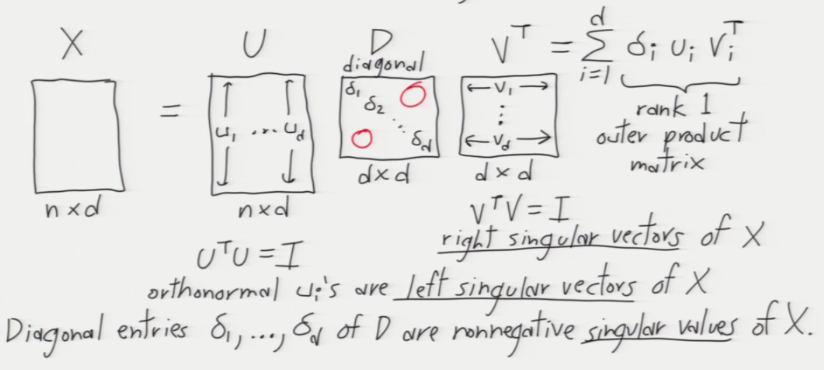
\includegraphics[scale=0.6]{../images/svd}
	\end{center}
	\item Poorly conditioned: look at biggest and smallest eigenvalues, divide.
	\item Fact: $v_{i}$ is an eigenvector of $X^{T}X$ with eigenvalue $\delta_{i}^{2}$.
	\item Proof: $X^{T}X = VDU^{T}UDV^{T} = VD^{2}V^{T}$ which is an eigen-decomposition of $X^{T}X$.
	\item Fact: We can find the $k$ greatest singular values and the corresponding vectors in $\bigo(ndk)$ time.
\end{itemize}

\subsection*{Clustering}
\begin{itemize}
	\item Partition data into clusters so points within a cluster are more similar than across clusters.
	\item Why?
	\begin{itemize}
		\item Discovery: find songs similar to songs you like; determine market segments.
		\item Hierarchy: Find good taxonomy of species from genes
		\item \underline{Quantization}: Compress a data set by reducing choices.
		\item \underline{Graph partitioning}: Image segmentation; find groups in social network.
		\begin{center}
			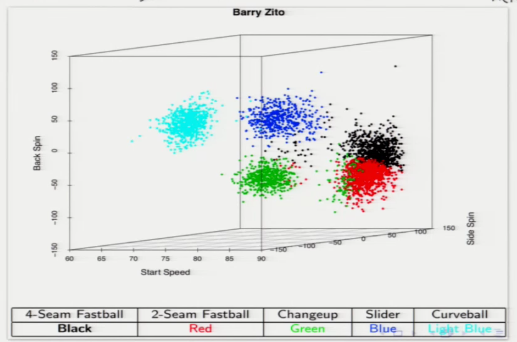
\includegraphics[scale=0.5]{../images/baseballclustering}
		\end{center}
	\end{itemize}
\end{itemize}
\subsubsection*{k-Means Clustering aka Lloyd's Algoritm}
\begin{itemize}
	\item Goal: Partition $n$ points into $k$ disjoint clusters. Assign each input point $X_{i}$ a cluster label $y_{i} \in [1, k].$
	\item Cluster $i'$s \underline{mean} is $\mu_{i} = \frac{1}{n_{i}} \sum_{y_{j}=i} X_{j}$, where $n_{i} =$ \# of points in $i$.
		\begin{center}
		\begin{tabular}{|c|}
			\hline
			Find $y$ that minimizes $\sum_{i=1}^{k} \sum_{y_{j}=i} |X_{j} - \mu_{i}|^{2}$\\
			\hline
		\end{tabular}
		\end{center}
	\item NP-Hard problem. Solvable in $\bigo(nk^{n})$ time.
	\item k-means heuristic: Alternate between:
		\begin{enumerate}
			\item $y_{j}$'s are fixed; update $\mu_{i}$'s.
				\begin{itemize}
					\item One can show (w/calculus) the optimal $\mu_{i}$ is the mean of the points in cluster $i$.
				\end{itemize}
			\item $\mu_{i}$'s are fixed; update $y_{j}$'s.
				\begin{itemize}
					\item The optimal $y$ assigns each point $X_{j}$ to closest center $\mu_{i}$.
				\end{itemize}
		\end{enumerate}
		Halt when step 2. changes no assignments.
		\begin{center}
			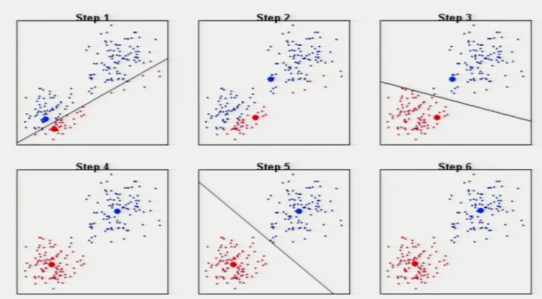
\includegraphics[scale=0.5]{../images/kmeansexample}
		\end{center}
		\item Both steps decrease objective function unless they change nothing. We never revisit the same set of assignments.
		\item Hence algorithm must terminate.
		\item Usually very fast in practice.
		\item Finds a local minimum, often not global.
		\item Getting started:
			\begin{itemize}
				\item Forgy method: Choose k random sample points to be initial $\mu_{i}$'s; go to step 2.
				\item Random partition: randomly assign each sample point to a cluster; go to step 1.
			\end{itemize}
		\item For best results, run k-means multiple times with random starts.
		\item Equivalent objective function: the \underline{within-cluster variation}
			\begin{center}
		\begin{tabular}{|c|}
			\hline
			Find $y$ that minimizes $\sum_{i=1}^{k} \frac{1}{n_{i}}\sum_{y_{j}=i}\sum_{y_{m}=i} |X_{j} - X_{m}|^{2}$ \\
			\hline
		\end{tabular}
		\end{center}
		\item Normalize the data? Same advice as for PCA. 
\end{itemize}

\subsubsection*{k-Medoids Clustering}
\begin{itemize}
	\item Generalizes k-means beyond Euclidean distance.
	\item Specify a \underline{distance function} $d(x, y)$ between points $x, y$ aka \underline{dissimilarity}.
	\item Can be arbitrary; ideally satisfies triangle inequality, $d(x, y) \leq d(x, z) + d(z, y)$.
	\item Replace mean computation with \underline{medoid}, the sample point that minimizes total distance to other points in same cluster.
\end{itemize}

\subsubsection*{Hierarchical Clustering}
\begin{itemize}
	\item Creates a tree; every subtree is a cluster.
	\item Bottom-up, aka \underline{agglomerative clustering}:
		start with each point a cluster; repeatedly \underline{fuse} pair of clusters.
	\item Top-down, aka \underline{divisive clustering}:
		start with all points in one cluster; repeatedly split it.
		We need a distance function for clusters A, B:
		\begin{itemize}
			\item \underline{complete linkage}: $d(A, B) = \max \{ d(w,x): w \in a, x \in B\}$.
			\item \underline{single linkage}: $d(A, B) = \min \{ d(w,x): w \in a, x \in B\}$.
			\item \underline{average linkage}: $d(A, B) = \frac{1}{|A||B|} \sum_{w \in A} \sum_{x \in B} d(w, x)$.
			\item \underline{centroid linkage}: $d(A, B) = d(\mu_{A}, \mu_{B})$.
		\end{itemize}
	\item Greedy agglomerative algorithm:
		\begin{itemize}
			\item Repeatedly \underline{fuse} the 2 clusters that minimize $d(A, B)$. Naively takes $\bigo(n^{3})$ time.
		\end{itemize}
	\item \underline{Dendrogram}: Illustration of cluster hierarchy (tree) in which the vertical axis encodes all the linkage distances.
		\begin{center}
			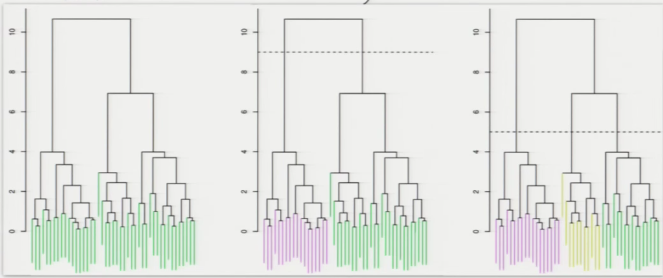
\includegraphics[scale=0.6]{../images/dendrogram}
			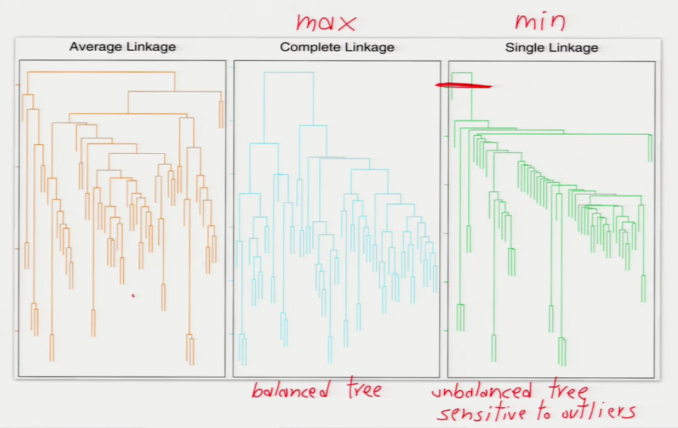
\includegraphics[scale=0.6]{../images/linkagedendrograms}
		\end{center}
	\item Warning: centroid linkage can cause \underline{inversions} where a parent cluster is fused at a lower height than its children.
\end{itemize}
\end{document}










